\section{Discussion}
In addition to the expert comments on ease of use and interpretability, we found that Tessevolve provides novel insight about which landscape dynamics may change as dimensions increase, and which may remain constant. In particular, we found that Tessevolve allowed us to see that, for the landscapes used here, \textit{landscape ruggedness} remains relatively unchanged as dimensions increase, but the ability to perform \textit{valley-crossing} greatly increases.

\subsection{Landscape Ruggedness}

Landscape ruggedness is a measure of how quickly fitness changes across a landscape. In smooth landscapes, points that are close together in evolutionary space will have similar fitness values. However, in very rugged landscapes, close points could have very different fitness values. 

\begin{figure}
    \centering
    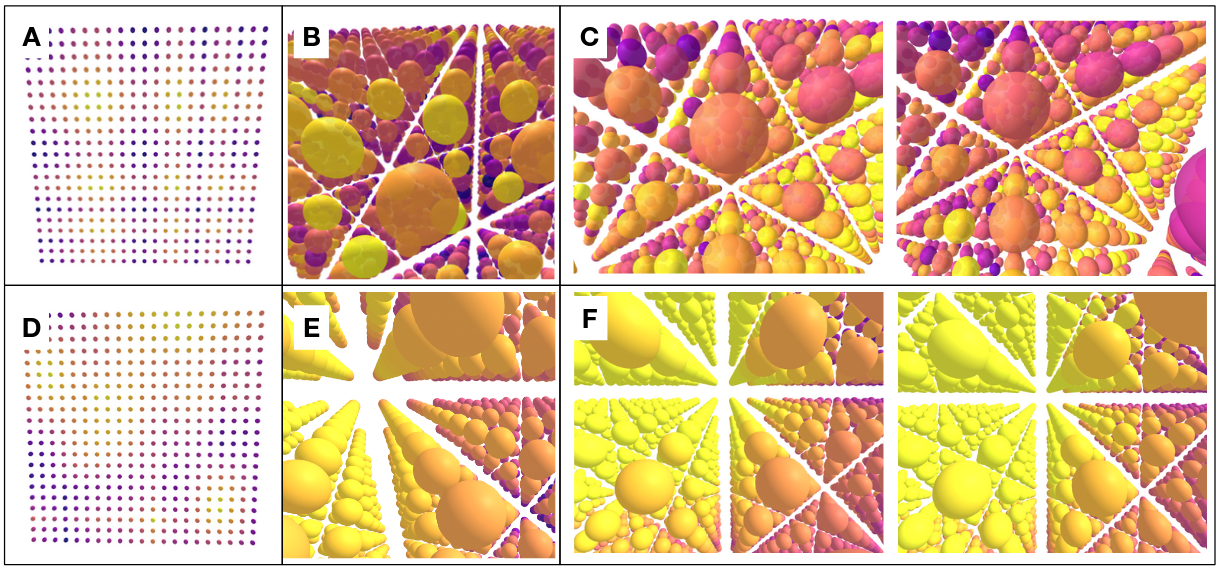
\includegraphics[width=0.5\textwidth]{chapters/3-vr-viz/figs/rugged.png}
    \caption{Ruggedness in Vincent (top) and Composite Fitness 1 (bottom) landscape. Note how properties of ruggedness transfer across dimensions. (A,D) 2-Dimensional landscape. (B,E) 3-Dimensional landscape. (C,F) Adjacent slices of 4-Dimensional landscape. }
    \label{fig:disc:rugged}
\end{figure}

The visual, color-based display of Tessevolve allowed us to see that landscapes which are rugged in lower dimensions also tend to be rugged in higher dimensions (\autoref{fig:disc:rugged}). This is mathematically unsurprising but previously difficult to visually demonstrate. Here, a smooth color gradient either across space (for 2D or 3D) or on scrolling (for 4D) easily maps to the concept of a smooth fitness gradient; similarly, colors that change very rapidly for adjacent spheres or slices are visually easy to notice and therefore easy to draw intuition about. This visual depiction of landscape ruggedness across dimensions helps reinforce intuition about how similar in fitness two similar trait states might be in higher-dimensional landscapes, even when we only have lower dimensional analogues. 

\subsection{Valley-Crossing in 2D vs. 3D vs. 4D}

\begin{figure}
    \centering
    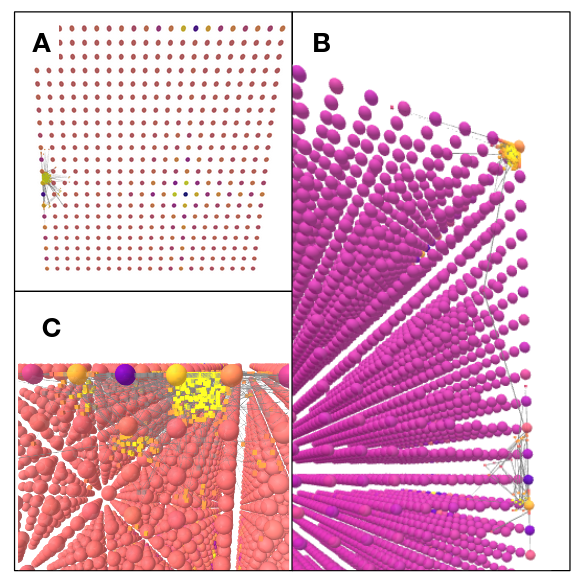
\includegraphics[width=0.5\textwidth]{chapters/3-vr-viz/figs/valley.png}
    \caption{Representative valley-crossing dynamics in 2D, 3D, and 4D. In each case, the Shubert function is the underlying evolutionary landscape, and populations mutate every generation with a standard deviation of 0.0001 and tournament size 16. The only difference in each is case is the number of dimensions. (A) 2D lineage where no valley-crossing occurs. (B) 3D lineage where valley-crossing occurs once across a large valley. (C) 4D lineage where the lineage stays primarily near one peak, but hops around nearby peaks frequently. }
    \label{fig:disc:valleys}
\end{figure}

In contrast to landscape ruggedness, one landscape feature that changed dramatically across landscapes was ease of landscape traversal and particularly ease of valley-crossing. As noted earlier, valley crossing is of particular interest because it helps to explain how populations transition from local optima to global optima. Here, the ability to visualize a lineage evolving across both a 2D and 3D landscape in multiple replicates demonstrates a quantitative difference in landscape traversal between replicates. For one set of parameters displayed in \autoref{fig:disc:valleys}, valley crossings from optimum to optimum occurred in 0 out of 10 replicates, while in 3D landscapes, they occurred in 8 out of 10 replicates. In all eight of these transitions, there was only a single valley crossing observed in the 1000 generations, and these peaks tended to be reasonably far apart (approximately half the distance of the entire landscape).

In 4D, however, rather than a single valley crossing from a one local optima to another, lineages tended to ``bounce" around closer peaks  multiple times across their evolutionary history. While there were some ``major" valley crossing as in 3D, the dominant dynamic was these more ``minor" crossings. 

The dynamics underlying these major vs.~minor valley crossings are not obvious from the visualization, nor are they intended to be; however, this visualization provides the insight that examining these large or small crossings might change across dimensions. 